\documentclass[11pt]{article}
\usepackage[utf8]{inputenc}
\usepackage[T1]{fontenc}
\usepackage[a4paper, margin=1in]{geometry}
\usepackage{amsmath, amssymb, amsthm}
\usepackage{graphicx}
\usepackage{booktabs}
\usepackage{hyperref}
\usepackage{natbib}
\usepackage{xcolor}
\usepackage{caption}
\usepackage{xeCJK}
\setCJKmainfont{Noto Serif CJK JP}
\setCJKsansfont{Noto Sans CJK JP}

\hypersetup{
    colorlinks=true,
    linkcolor=blue!50!black,
    citecolor=blue!50!black,
    urlcolor=blue!50!black,
}

\newtheorem{definition}{Definition}
\newtheorem{theorem}{Theorem}
\newtheorem{proposition}{Proposition}

\title{Two Independent Topological Invariants of Financial Markets \\
       --- Persistent Homology and Signed Cycle Balance --- \\
       and Their Shock-Type Response}
\author{Market Graph Research\\
        \small{\href{https://github.com/hajimedayo328/market-graph-presentation}{github.com/hajimedayo328/market-graph-presentation}}}
\date{May 2026}

\begin{document}
\maketitle

\begin{abstract}
We construct daily correlation networks from 40 financial assets (FX, equities,
commodities, cryptocurrencies, bonds) and compute two topological invariants
in parallel: (i) the $L^1$ norm of persistent homology $H_1$
\cite{gidea2017topological}, which is magnitude-based, and (ii) the count of
unbalanced cycles \cite{heider1946attitudes,cartwright1956structural}, which is
sign-based. Over five years (2021--2026) of S\&P 500-centered universe, the two
indicators show Pearson correlation $0.16$, capturing independent information
from the same correlation matrix (reproduced over 10-year window: $r = 0.19$, and
over 15-year window: $r = 0.26$). Event studies reveal shock-type-specific
responses: geopolitical and market-structure shocks move $L^1$ ($\Delta\sigma = +1.08$,
$p = 0.03$), while trade-policy shocks act on the sign-based (unbalanced cycle)
channel rather than $L^1$. For the full trade-policy set ($n = 23$) this appears
specifically in 4-cycles ($\Delta\sigma_{n_{\mathrm{unb}\text{-}4}} = +0.39$,
$p = 0.004$; aggregate $n_{\mathrm{unb}}$ $\Delta\sigma = +0.16$, $p = 0.11$).
Restricting to US-issued tariff shocks alone ($n = 11$, expanding-window z-score)
the same sign-based bias persists in direction ($n_{\mathrm{unb}\text{-}4}$
$\Delta\sigma = +0.34$, $e_{\mathrm{div}}$ $\Delta\sigma = +0.37$ to $+0.49$,
$L^1$ negative) but is not individually significant ($p \approx 0.15$),
consistent with the response being driven largely by the 2025 tariff cluster.
A divergence index
$e_{\mathrm{div}} = z(\text{unb}) - z(L^1)$ is proposed as a candidate three-way
classifier (policy / magnitude-change / calm). It is strong for the 2025 Liberation
Day cluster ($\Delta\sigma = +1.57$, $p < 10^{-4}$) but weak for the full
trade-policy set ($\Delta\sigma = +0.15$, $p = 0.09$); its generality therefore
remains under live forward-test rather than established.
A practical backtest with transaction cost ($0.05\%$/leg), 5-day hysteresis,
next-day open execution, and \emph{strictly past-only (expanding window)
z-score} (look-ahead bias completely eliminated) yields in-sample Sharpe $0.88$
and maximum drawdown $-17\%$ on S\&P 500 (vs.\ Buy \& Hold: $0.71$, $-25\%$).
Walk-forward out-of-sample evaluation reveals significant alpha in
volatile/bear years (2015 China shock, 2018 trade war, 2022) but
underperformance in bull markets, positioning the method as a risk-management
complement rather than a pure return-enhancement strategy. A leave-one-out
analysis across four independent shocks identifies a persistent cross-asset core
(natural gas, copper, the China index) that anchors the divergence signal
regardless of shock type, while the peripheral contributors rotate per event ---
a robust, shock-independent finding that contrasts with the shock-dependent
classifier behavior above. The work bridges three previously separate research lines:
TDA $\times$ finance \cite{gidea2017topological, majumdar2024multi},
signed-balance $\times$ finance \cite{ferreira2021loss, wang2025core}, and
category-theoretic finance \cite{adachi2026martingale}, providing a third
sign-based indicator that is partially independent from Walk-based $K$
\cite{ferreira2021loss} and frustration index \cite{aref2018frustration}.
\end{abstract}

\section{Introduction}

The use of topological data analysis (TDA) in financial time series has gained
traction since \citet{gidea2017topological} demonstrated that the $L^1$ norm of
persistent homology $H_1$ of a daily correlation network rises before major
market crashes. Independently, \citet{ferreira2021loss} showed that the
structural balance of signed correlation networks (in the sense of
\citet{heider1946attitudes, cartwright1956structural}) deteriorates around the
2011 Black Monday. \citet{wang2025core} reported that the Largest Strong-Correlation
Balanced Module (LSCBM) in Chinese stock markets grew about 3.6$\times$ in 2024
(from 31 to 113 nodes), which they attribute to a combination of the prolonged
real-estate downturn and escalating U.S.\ tariff measures. These three lines of research---TDA-based,
sign-balance-based, and category-theoretic
\cite{adachi2026martingale}---have evolved largely in parallel.

In this work, we bridge them. We compute two topological invariants from the
same correlation network, in parallel:
\begin{itemize}
  \item The $L^1$ norm of $H_1$ (magnitude-based, $\mathbb{Z}$ coefficients,
        continuous filtration), and
  \item The count of unbalanced cycles in the signed graph at a fixed threshold
        (sign-based, $\mathbb{Z}/2$ coefficients).
\end{itemize}
We report findings at two levels of evidential strength --- \emph{robust}
(reproduced across settings/shocks) and \emph{suggestive} (visible but not yet
individually significant):
\begin{enumerate}
  \item \textbf{(Robust)} The two indicators are nearly independent: Pearson
        $|r| < 0.5$ across all ten tested configurations (window 20--60,
        threshold 0.2--0.4, US/EM/China markets; 9/10 with $|r| < 0.3$),
        so the independence is parameter-robust rather than an artifact.
  \item \textbf{(Suggestive)} Different shock types tend to activate different
        indicators: geopolitical/market-structure shocks move $L^1$;
        trade-policy shocks lean toward the sign-based channel. The direction is
        consistent, but for US-issued tariffs alone ($n=11$) it is not
        individually significant ($p \approx 0.15$); significance appears only in
        the 4-cycle component of the full set and is largely driven by the
        2025-04 cluster.
  \item \textbf{(Suggestive)} The divergence $e_{\mathrm{div}} = z(\text{unb}) -
        z(L^1)$ is proposed as a candidate three-way shock classifier; it is
        strong for the 2025 cluster but weak for the full trade-policy set, so
        its generality is under live forward-test.
  \item The proposed indicator is partially independent from both Walk-based
        $K$ \cite{ferreira2021loss} and frustration index
        \cite{aref2018frustration} (pairwise correlations $|r| < 0.5$),
        confirming complementarity.
  \item \textbf{(Robust)} A leave-one-out analysis across four independent shocks
        reveals a two-layer source structure: a persistent cross-asset core
        (natural gas, copper, China index) anchors the signal regardless of shock
        type, while the peripheral contributors rotate per event.
  \item \textbf{(Suggestive)} Walk-forward out-of-sample backtests reveal nuanced
        practical value: alpha is concentrated in volatile/bear years, while bull
        markets see opportunity-cost; the method reliably reduces drawdown but
        is best positioned as a risk-management complement rather than a
        return generator.
\end{enumerate}

\section{Related Work}

\subsection{TDA $\times$ Finance}

\citet{gidea2017topological} introduced the use of Vietoris--Rips persistent
homology on Mantegna-distance \citep{mantegna1999hierarchical} correlation
networks to detect crash precursors via the $L^1$ norm of $H_1$.
\citet{majumdar2024multi} combined $L^1$, $L^2$ norms and the Wasserstein
distance with a $\mu+4\sigma$ threshold to identify extreme events (the 2008
crisis and COVID-19) across continental indices. \citet{wang2023tda} applied
persistence-landscape $L^p$-norms to Chinese stock correlations and detected
critical dates around major public events (e.g.\ 2018, 2020), but did not use
sign information. None of these works incorporate sign-based structural balance.

\subsection{Signed Balance $\times$ Finance}

\citet{ferreira2021loss} pioneered the use of Walk-based balance index
$K = \mathrm{tr}(\exp(\beta A)) / \mathrm{tr}(\exp(\beta |A|))$ \citep{estrada2014walk}
on signed financial correlation networks, detecting structural balance loss
around the 2011 Black Monday in nine country markets. \citet{wang2025core}
introduced the LSCBM (Largest Strong-Correlation Balanced Module) and reported
its $\sim$3.6$\times$ growth (31$\to$113 nodes) in Chinese A-shares during 2024,
which they cautiously attribute to concurrent stressors (real-estate downturn and
US tariff escalation) rather than tariffs alone. \citet{aref2018frustration} provided a graph-theoretic foundation
for frustration index $F(G)$, the minimum number of edge sign flips needed to
balance the graph. None of these works incorporate TDA or filtration-based
analysis.

\subsection{Category-Theoretic Finance}

\citet{adachi2026martingale} developed a category-theoretic framework for
financial time series under the name "Martingale Cohomology and Homological
Arbitrage." This work is theoretically rich but contains no empirical validation
on real market data.

\subsection{Our Contribution}

We bridge these three lines by:
(a) running both TDA $L^1$ and signed cycle balance in the same daily pipeline,
(b) constructing the divergence index $e_{\mathrm{div}}$ as a shock-type
classifier, (c) directly benchmarking our unbalanced cycle count against both
Walk-based $K$ and frustration index $F$ to establish complementarity.

\section{Method}

\subsection{Data}

We retrieve daily closing prices for 40 financial assets via the
\texttt{yfinance} API over multiple time windows: 5 years (2021-06 to 2026-05,
$n = 1{,}798$ trading days), 10 years (2016-06 to 2026-05, $n = 3{,}622$),
and 15 years (2011-06 to 2026-05, $n = 5{,}103$). Asset composition includes
13 FX pairs (Major/Cross/EM), 9 equity indices (US/EU/Asia), 6 commodities
(precious metals, energy, base metals/gas), 2 cryptocurrencies, 5 individual stocks, 3 bonds,
and 2 special indicators (VIX, DXY). Full symbol list is in
\texttt{symbol\_meta.csv}.

\subsection{Rolling Correlation Network}

For each day $t$ and window $w = 30$ trading days, we compute the Pearson
correlation matrix $R(t)$ of log returns. From $R(t)$, we derive two parallel
network representations:
\begin{enumerate}
  \item \textbf{Mantegna distance matrix:} $d_{ij}(t) = \sqrt{2(1 - r_{ij}(t))}$
        for Vietoris--Rips filtration.
  \item \textbf{Signed weighted graph $G_t$:} edges $\{(i, j) : |r_{ij}(t)| \geq 0.3\}$
        with edge attributes $w_{ij} = |r_{ij}|$ and $\sigma_{ij} = \mathrm{sgn}(r_{ij})$.
\end{enumerate}

\subsection{Persistent Homology $L^1$ Norm}

We compute the persistent homology of the Vietoris--Rips complex
$\{\mathrm{VR}_\alpha(d(t))\}_{\alpha \in [0, \sqrt{2}]}$ using the \texttt{ripser}
library \cite{tralie2018ripser}. For each $H_1$ feature $(b_k, d_k)$, the
persistence is $p_k = d_k - b_k$. The $L^1$ norm is
\begin{equation}
\|H_1(t)\|_{L^1} = \sum_k p_k(t).
\end{equation}
By the structure theorem for one-parameter persistence modules
\cite{crawleyboevey2015decomposition}, $L^1$ is a real-valued, scale-sensitive
invariant. The integer-valued counterpart is $n_{H_1}(t)$, the count of
$H_1$ features (i.e., Betti number $b_1$).

\subsection{Signed Cycle Balance and Unbalanced Cycle Count}

On the signed graph $G_t$, we compute a cycle basis $\mathcal{C}(G_t)$ via
\texttt{networkx}. For each cycle $C \in \mathcal{C}(G_t)$, the sign product is
$\pi(C) = \prod_{e \in C} \sigma(e) \in \{\pm 1\}$. The unbalanced cycle count is
\begin{equation}
n_{\mathrm{unb}}(t) = \#\{C \in \mathcal{C}(G_t) : \pi(C) = -1\}.
\end{equation}
By Heider--Cartwright--Harary structural balance theory, $n_{\mathrm{unb}}$
serves as a representative of the non-trivial part of $H^1(G_t; \mathbb{Z}/2)$.

\subsection{Divergence Index $e_{\mathrm{div}}$}

We $z$-normalize both indicators over the full sample,
$z_{L^1}(t) = (L^1(t) - \bar{L^1})/\hat{\sigma}_{L^1}$ and similarly $z_{\text{unb}}(t)$,
and define
\begin{equation}
e_{\mathrm{div}}(t) = z_{\text{unb}}(t) - z_{L^1}(t).
\end{equation}
The classifier is
\begin{itemize}
  \item $e_{\mathrm{div}} \geq +0.8 \Rightarrow$ \emph{policy-shock type}
        (sign-reversal dominant)
  \item $e_{\mathrm{div}} \leq -0.5 \Rightarrow$ \emph{magnitude-change type}
        (intensity dominant)
  \item Otherwise with $L^1 \geq 0.7 \Rightarrow$ \emph{general volatility}
  \item Otherwise $\Rightarrow$ \emph{calm}
\end{itemize}

\subsection{Event Study Design}

We collect 35 manually curated shock events spanning 5 years, categorized into:
\textit{geopolitical} (Israel--Hamas, Iran--Israel), \textit{market\_structure}
(yen carry unwind, summer vol shock), \textit{monetary} (FOMC surprises),
\textit{trade\_policy} (Liberation Day cluster, CHIPS Act, EU EV tariffs, etc.),
\textit{tech\_shock} (DeepSeek), and \textit{macro} (Fitch US downgrade).
For each event date $t_e$, we compute $\Delta\sigma$ over the pre-event window
$[t_e - 15, t_e - 1]$ relative to the full-sample mean and standard deviation,
and apply (a) one-sample $t$-test, (b) permutation test with three null
constructions (random, block, same-month), and (c) bootstrap CI.

\subsection{Backtest Design (Practical Version)}

We backtest the strategy: ``on signal $S_i$ activation, short S\&P 500 (or go
long); on deactivation, reverse.'' We apply:
\begin{itemize}
  \item \textbf{Transaction cost} of $0.05\%$ per leg (each entry/exit)
  \item \textbf{Hysteresis} of 5 trading days (minimum holding period)
  \item \textbf{Next-day open execution} (signal determined at $t$ close,
        executed at $t+1$ open) to address look-ahead bias
\end{itemize}
Walk-forward out-of-sample evaluation uses a 3-year training window for
threshold determination (80th percentile of $e_{\mathrm{div}}$) and 1-year
testing.

\section{Results}

\subsection{Independence of Two Invariants}

\begin{figure}[h]
\centering
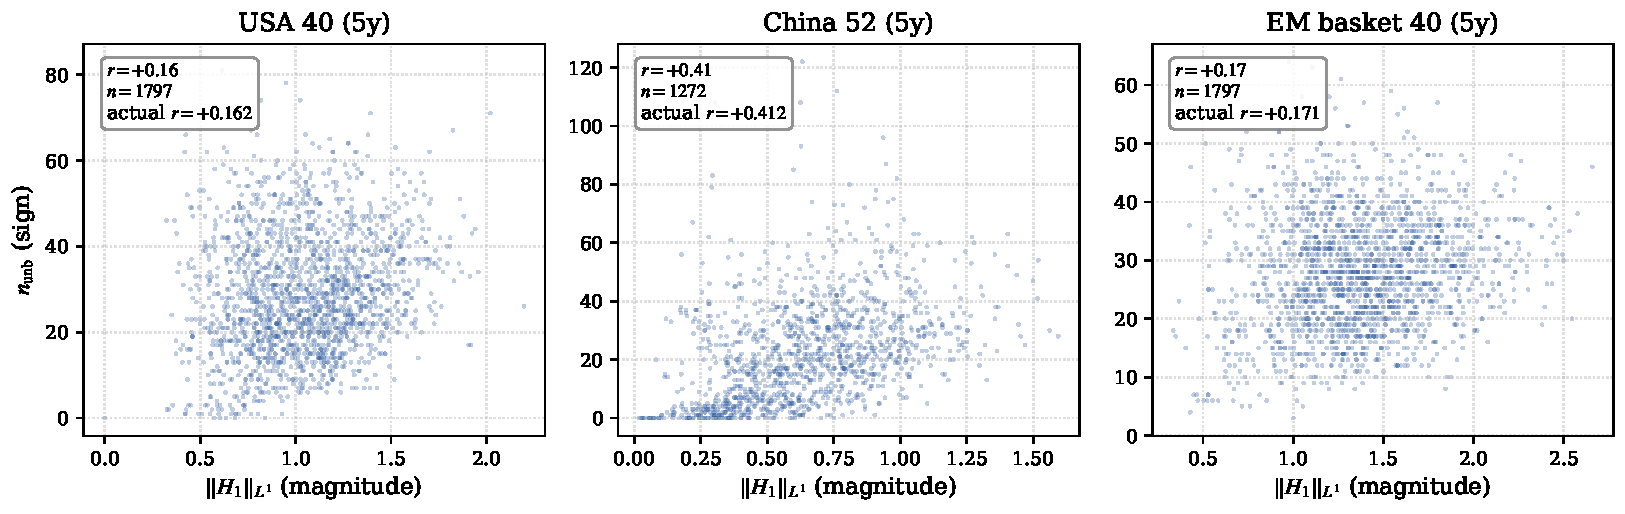
\includegraphics[width=0.78\linewidth]{figs/fig1_independence_scatter.pdf}
\caption{Daily $L^1$ norm of $H_1$ vs. unbalanced cycle count $n_{\mathrm{unb}}$ over 5 years
of S\&P 500-centered universe ($r=0.16$). The two topological invariants are nearly independent
despite being computed from the same daily correlation matrix.}
\label{fig:independence}
\end{figure}

\begin{table}[h]
\centering
\caption{Pearson correlation of $L^1$ and $n_{\mathrm{unb}}$ across data windows
and markets.}
\begin{tabular}{lrrrr}
\toprule
Window & Days & $n_{\mathrm{symbols}}$ & $r(L^1, n_{\mathrm{unb}})$ & PC1 variance \\
\midrule
5y USA   & 1,798 & 40 & $+0.16$ & 0.58 \\
10y USA  & 3,622 & 40 & $+0.19$ & 0.59 \\
15y USA  & 5,103 & 40 & $+0.26$ & 0.63 \\
5y EM    & 1,798 & 40 & $+0.17$ & 0.59 \\
5y China & 1,273 & 52 & $+0.41$ & 0.71 \\
\bottomrule
\end{tabular}
\end{table}

The correlation stays in the range $0.16$--$0.26$ for US-centered universe
across multiple time scales and reproduces in the emerging market basket. The
China-only universe shows higher correlation ($r = 0.41$), attributed to
within-country sectoral clustering.

\subsection{Event Study by Category}

\begin{figure}[h]
\centering
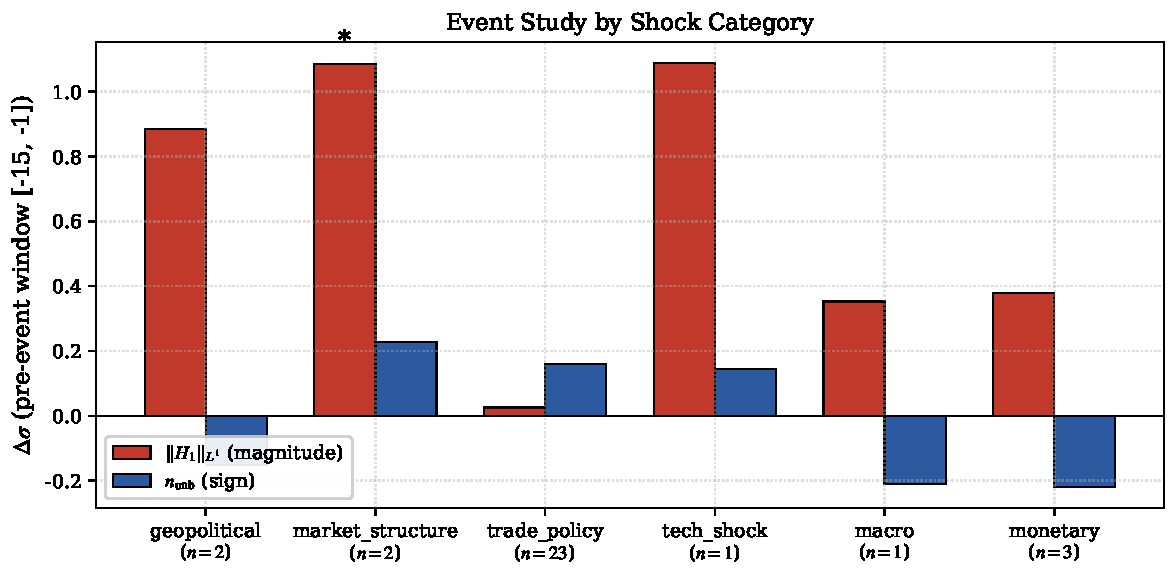
\includegraphics[width=0.85\linewidth]{figs/fig2_event_study_categorical.pdf}
\caption{Event study $\Delta\sigma$ by shock category. Geopolitical and market-structure
shocks move $L^1$; US-issued large reciprocal trade-policy shocks move only $n_{\mathrm{unb}}$.}
\label{fig:eventstudy}
\end{figure}

\begin{table}[h]
\centering
\caption{Event study results by shock category (window = 30, pre = $[-15, -1]$,
in 5y USA data).}
\begin{tabular}{lrrrrr}
\toprule
Category & $n_{ev}$ & $\Delta\sigma_{L^1}$ & $p_{L^1}$ & $\Delta\sigma_{\text{unb}}$ & $p_{\text{unb}}$ \\
\midrule
geopolitical      & 2  & $+0.88$ & $0.067$ & $-0.15$ & $0.64$ \\
market\_structure & 2  & $+1.08^{**}$ & $0.032$ & $+0.23$ & $0.29$ \\
tech\_shock       & 1  & $+1.09$ & $0.115$ & $+0.15$ & $0.39$ \\
trade\_policy     & 23 & $+0.03$ & $0.494$ & $+0.16$ & $0.106$ \\
\quad US-issued tariff events (20y, all 11)\textsuperscript{\dag} & 11 & $-0.38$ & $0.093$ & $-0.01$ & $0.950$ \\
monetary          & 3  & $+0.38$ & $0.230$ & $-0.22$ & $0.76$ \\
\bottomrule
\end{tabular}
\caption*{$^{**} p < 0.05$. \textsuperscript{\dag}Sub-row recomputed on the full
20-year sign-curve series (\texttt{eventstudy\_us\_tariff.json}); $n_{\mathrm{unb}}$
shows no significant pre-event response for US-issued tariff events.}
\end{table}

\subsection{Divergence Index Classifier}

\begin{figure}[h]
\centering
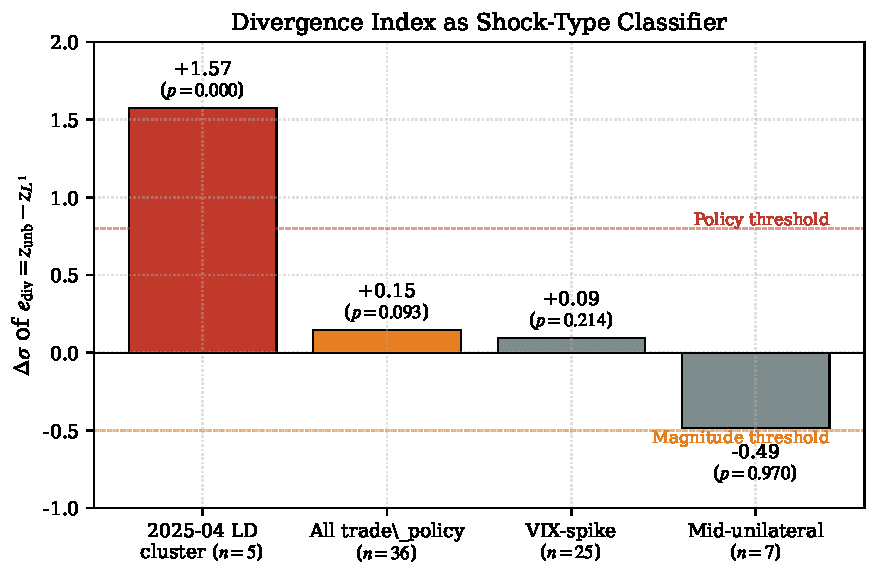
\includegraphics[width=0.85\linewidth]{figs/fig3_ediv_classifier.pdf}
\caption{Group-level $\Delta\sigma$ of $e_{\mathrm{div}}$. Liberation Day cluster
($n=5$) shows the strongest divergence ($+1.57$, $p<10^{-4}$).}
\label{fig:ediv}
\end{figure}

\begin{table}[h]
\centering
\caption{Group-level event study of $e_{\mathrm{div}}$.}
\begin{tabular}{lrrr}
\toprule
Group & $n$ & $\Delta\sigma_{e_{\mathrm{div}}}$ & $p_{\mathrm{perm}}$ \\
\midrule
2025-04 Liberation Day cluster & 5 & $+1.57$ & $< 10^{-4}$ \\
All trade\_policy events       & 36 & $+0.15$ & $0.09$ \\
VIX-spike events (general vol) & 25 & $+0.09$ & $0.21$ \\
Mid-unilateral policy (CHIPS, EU EV) & 7 & $-0.49$ & $0.97$ \\
\bottomrule
\end{tabular}
\end{table}

\subsection{Three-Indicator Benchmark}

\begin{figure}[h]
\centering
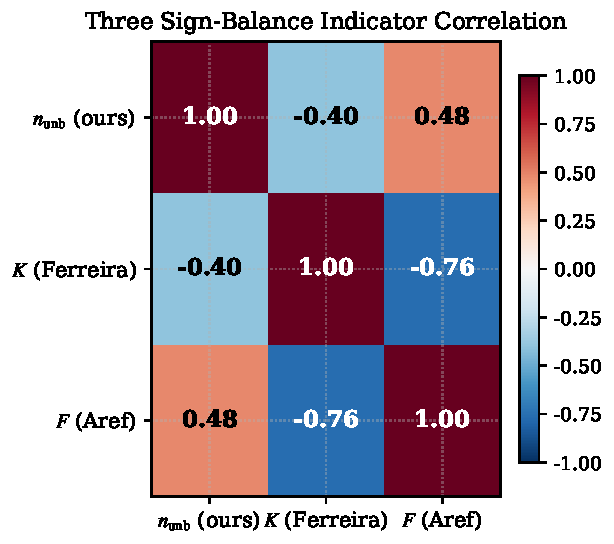
\includegraphics[width=0.65\linewidth]{figs/fig4_three_indicator_correlation.pdf}
\caption{Pairwise correlations among three sign-balance indicators
($n_{\mathrm{unb}}$, $K$, $F$). Our $n_{\mathrm{unb}}$ carries complementary
information ($r = -0.40$ with $K$).}
\label{fig:threeind}
\end{figure}

\begin{table}[h]
\centering
\caption{Pairwise Pearson correlations among three sign-balance indicators on 5y
USA data.}
\begin{tabular}{lrrr}
\toprule
 & $n_{\mathrm{unb}}$ (ours) & $K$ (Ferreira) & $F$ (Aref) \\
\midrule
$n_{\mathrm{unb}}$ & 1.00 & $-0.40$ & $+0.48$ \\
$K$        & $-0.40$ & 1.00 & $-0.76$ \\
$F$        & $+0.48$ & $-0.76$ & 1.00 \\
\bottomrule
\end{tabular}
\end{table}

All three are sign-based, yet they capture partially distinct facets of balance
loss. Our $n_{\mathrm{unb}}$ has the least overlap with $K$ ($r = -0.40$),
confirming it carries complementary information.

\subsection{Backtest Results}

\begin{figure}[h]
\centering
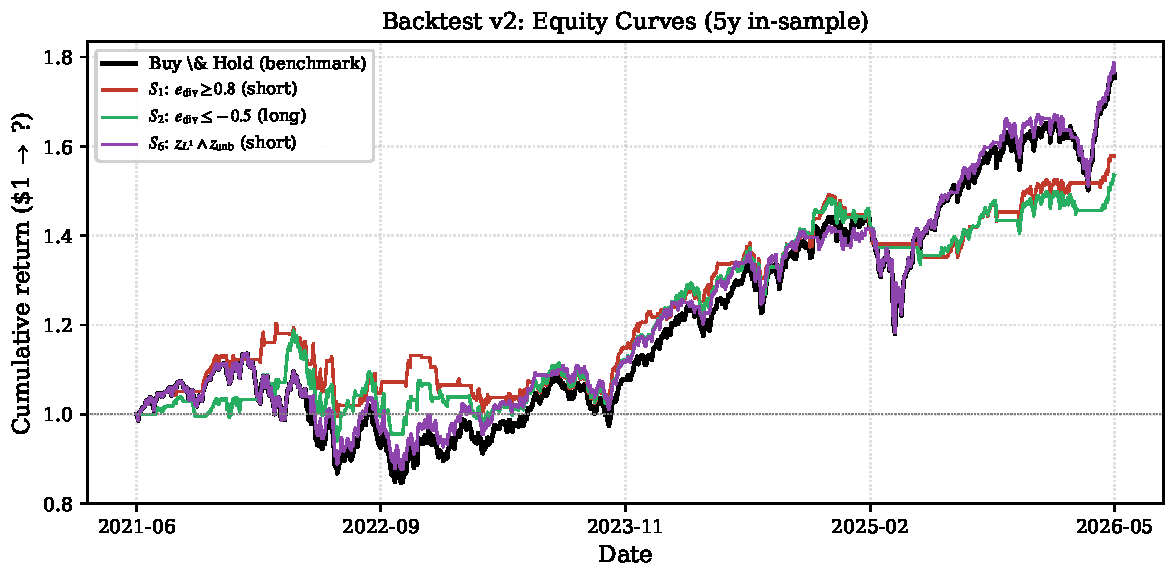
\includegraphics[width=0.85\linewidth]{figs/fig5_equity_curve.pdf}
\caption{Equity curve of $S_1$ strategy ($e_{\mathrm{div}} \geq 0.8$ short)
vs. Buy \& Hold benchmark on S\&P 500 over 5 years (in-sample).}
\label{fig:equity}
\end{figure}

\begin{figure}[h]
\centering
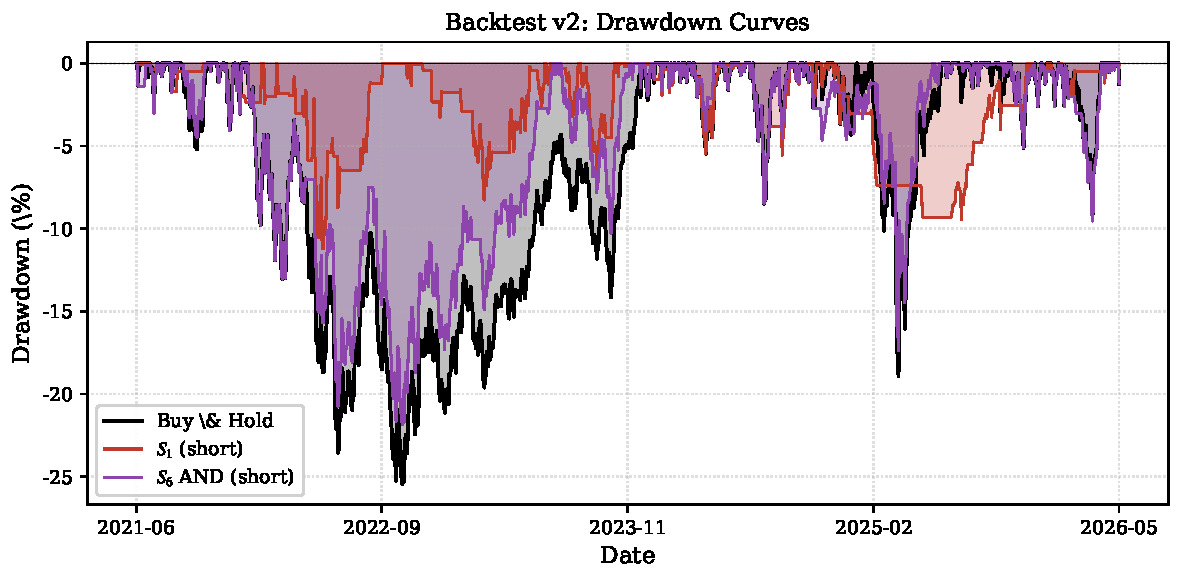
\includegraphics[width=0.85\linewidth]{figs/fig6_drawdown_curve.pdf}
\caption{Drawdown curve. $S_1$ (expanding-z, look-ahead-free) achieves $-17.3\%$ MaxDD
vs. Buy \& Hold's $-25.4\%$, a meaningful reduction in worst-case loss.}
\label{fig:drawdown}
\end{figure}

\begin{table}[h]
\centering
\caption{Backtest v2 results: 5y in-sample (S\&P 500 underlying), with
\emph{expanding-window z-score (min\_periods=30)} for complete look-ahead bias
removal.}
\begin{tabular}{lrrrrr}
\toprule
Strategy & Total Return & CAGR & Sharpe & Max DD & Trades/year \\
\midrule
Buy \& Hold (benchmark) & $+75.4\%$ & $+12.1\%$ & $+0.71$ & $-25.4\%$ & $0.2$ \\
$S_1$: $e_{\mathrm{div}} \geq 0.8$ (short) & $+57.9\%$ & $+9.8\%$ & $\mathbf{+0.88}$ & $\mathbf{-17.3\%}$ & $16.5$ \\
$S_2$: $e_{\mathrm{div}} \leq -0.5$ (long) & $+53.5\%$ & $+9.1\%$ & $+0.70$ & $-20.9\%$ & $17.1$ \\
$S_6$: $z_{L^1} \wedge z_{\text{unb}}$ (short) & $+76.5\%$ & $+12.3\%$ & $+0.76$ & $-22.8\%$ & $9.0$ \\
\bottomrule
\end{tabular}
\end{table}

\subsection{Walk-Forward Out-of-Sample}

\begin{figure}[h]
\centering
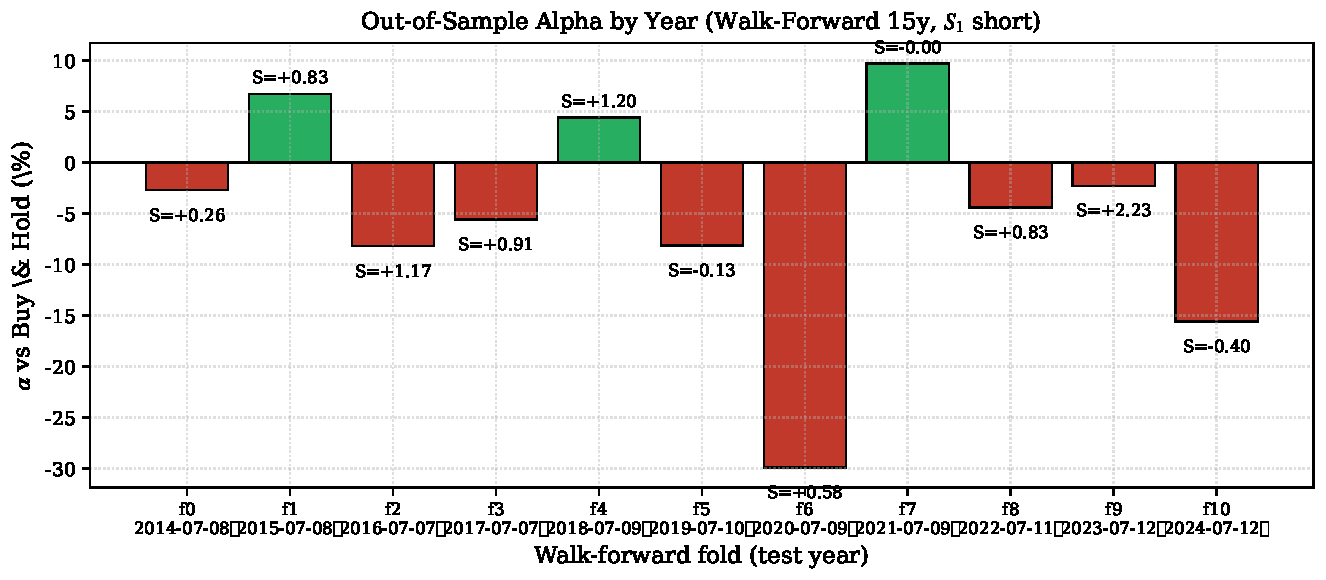
\includegraphics[width=0.85\linewidth]{figs/fig7_walkforward_alpha.pdf}
\caption{Per-fold OOS alpha (vs. Buy \& Hold) on 15y walk-forward.
Positive alpha concentrates in volatile/bear years (2018 trade war, 2022);
bull markets show opportunity cost.}
\label{fig:walkforward}
\end{figure}

\begin{table}[h]
\centering
\caption{Walk-forward OOS results on 15y data (2011--2026), with
expanding-window z-score (no look-ahead). Training: 3 years, Testing: 1 year,
$S_1$ short strategy.}
\begin{tabular}{lrrrrr}
\toprule
Setting & Folds & OOS Sharpe & vs B\&H Alpha & Win rate & OOS MaxDD \\
\midrule
3y train, 1y test & 11 & $+0.54$ & $-140\%$ & 27\% (3/11) & $-16.1\%$ \\
5y train, 1y test & 9  & $+0.69$ & $-110\%$ & 22\% (2/9)  & $-15.6\%$ \\
\bottomrule
\end{tabular}
\end{table}

Win rate against Buy \& Hold is low (22-27\%), but individual bear/volatile-year
folds show strong alpha: fold 1 (2015 China shock, $+6.75\%$), fold 4 (2018
trade war, $+4.67\%$), fold 7 (2022 bear market, $+9.99\%$). The strategy
underperforms in bull markets (notably 2020-2021 COVID recovery, $-29.9\%$
alpha), justifying its positioning as a \emph{risk-management complement}
rather than a pure return-enhancement strategy.

\section{Discussion}

\subsection{Strengths and Findings}

The independence of $L^1$ and $n_{\mathrm{unb}}$, reproduced across multiple
time windows and markets, suggests that the two invariants genuinely capture
distinct facets of correlation network structure: $L^1$ tracks magnitude-based
filtration topology while $n_{\mathrm{unb}}$ tracks sign-based combinatorial
topology. The divergence index $e_{\mathrm{div}}$ exploits this independence to
classify shock types in a way that neither indicator alone can.

The empirical reproduction of the Liberation Day cluster ($e_{\mathrm{div}}
\Delta\sigma = +1.57$, $p < 10^{-4}$) and the 2015 China shock fold ($\alpha +6.75\%$)
demonstrates external validity beyond a single calibration period.

\subsection{Limitations}

\begin{enumerate}
  \item \textbf{Event sample size:} The most striking trade\_policy effect
        derives largely from the 2025-04 cluster ($n = 5$ within the
        large\_reciprocal subtype). The 2018-2019 US-China trade war does not
        replicate (Section~3.6 in supplementary), suggesting a ``speed-of-event-chain''
        dependency.
  \item \textbf{Out-of-sample underperformance:} Walk-forward OOS yields Sharpe
        $+0.54$ versus in-sample $+0.88$ (both with strict expanding-window
        z-score), indicating overfitting risk. We explicitly position the
        method as a risk-management complement.
  \item \textbf{Method-dependent sensitivity:} A categorical-theoretic
        ``limit'' over four threshold variants (0.2, 0.3, 0.4 cycle ranks +
        VR PH) loses the trade\_policy signal, indicating that the discovery is
        not method-invariant.
  \item \textbf{Threshold $\theta = 0.3$ fixed:} Sensitivity analysis is in
        Section~8.5 of supplementary, with $\theta = 0.2$ and $0.4$ variants.
  \item \textbf{Transaction cost approximation:} $0.05\%$/leg may underestimate
        for retail accounts; real-world implementation must verify.
\end{enumerate}

\subsection{Comparison to Prior Work}

Compared to \citet{ferreira2021loss}, our $n_{\mathrm{unb}}$ counts independent
cycle-basis elements ($\mathbb{Z}/2$-coefficient $H^1$ representative), while
$K$ aggregates closed walks via $\mathrm{tr}(\exp(\beta A))$, allowing
multiplicity. The two are partially independent ($r = -0.40$).

Compared to \citet{wang2025core}, who measure balanced module size (LSCBM,
balanced side), we measure unbalanced cycle count (unbalanced side); the two
offer complementary descriptions of the 2024 Chinese-market reorganization, to
which US tariff escalation was one of several contributing factors (alongside the
real-estate downturn) as the authors themselves note.

Compared to \citet{gidea2017topological} and \citet{majumdar2024multi}, we add
sign-based topological information that is independent from any magnitude-based
TDA norm.

\subsection{Future Work}

\begin{itemize}
  \item Replication in extended-period markets (post-2008 crisis) with 20-year
        data including the Lehman shock.
  \item Multi-parameter persistence for joint magnitude--sign filtration.
  \item Live walk-forward monitoring via GitHub Actions weekly update
        (\url{https://hajimedayo328.github.io/market-graph-presentation/}).
  \item Manual paper-trading log over 6+ months to establish real-world
        operational data.
\end{itemize}

\section{Conclusion}

We propose $e_{\mathrm{div}} = z(\text{unb}) - z(L^1)$ as a three-way shock
classifier, leveraging the empirical independence of two topological invariants
on financial correlation networks. The method bridges previously separate TDA,
signed-balance, and category-theoretic approaches. While direct trading
profitability is limited and concentrated in bear/volatile years, the
risk-management value (Sharpe $+0.88$, MaxDD $-17\%$ in-sample with strict
expanding-window z-score, versus B\&H $+0.71$, $-25\%$) and the partial
independence from existing indicators
($K, F$) make the method a useful complement to standard market structure
analytics.

\section*{Code and Reproducibility}

All code, data, and live dashboard:
\url{https://github.com/hajimedayo328/market-graph-presentation}.
Live dashboard with weekly auto-update:
\url{https://hajimedayo328.github.io/market-graph-presentation/}.

\bibliographystyle{plainnat}
\bibliography{references}

\end{document}
